\chapter{Experiments}
\label{chap:experim}
%\section{Overview}
In this chapter will be shown all the experiments performed and their results. The first section starts from what we expect to show from experiments on code and, to this aim, what kind of comparisons will be made.\\
The second section will explain how to implement tests, ie chosen datasets for each type of code and scripts main features.
After that, the other section will move on results, in particular will be shown time measures and plots with some final remarks and comparisons with respect to what we expected.

%\section{What and How}
%What and How
\section{Expectations}
As previously mentioned, what we want to see is that our model and implementation of a Farm parallel pattern can fit in a GPU.
To this aim is necessary to gain a speedup in the order of the number of Streaming multiprocessors of the GPU we're running code.
Let's clarify some concepts in the sentence above:

\begin{itemize}
	\item The speedup will be estimated in terms of \textbf{GPU completion time}, ie the total time needed to perform all data transfers and kernel executions for a certain application;
	\item We expect to have the best speedup only when we have certain conditions;
	\item The best speedup for would be in the order of multiprocessors number.
\end{itemize}
The last point means we can't expect to reach greater gain than the available amount of hardware resources. This is strictly related to the fact that we can't expect Streaming parallel problems, that we implemented, to perform better than the equivalent Data Parallel version. \footnote{As we mentioned in previous Chapters, the GPU is specifically designed to be efficient and to perform at its best on Data Parallel problems.}
The second point above means we expect the best performances in the following cases:
\begin{itemize}
	\item When we have a regular kernel, that is a kernel with the lowest possible amount of branching and, thus, very low (or absent) threads divergence;
	\item When the kernel is more computational-bound than memory bound, the less access to Global memory the less data transfer latency will slow down computations;
	\item When the kernel execution takes an amount of time near the one for a data transfer.
\end{itemize} 
When one, or more, of the above conditions isn't meet we expect to have a considerably lower speedup.


\subsection{Measures: What and How}
Before the test setup and writing it's important to understand what we should measure, in order to get significant comparisons.\\
First we recall that the measures of interest are relative to \textit{data transfers} and \textit{kernel execution}. Clearly, in the case were CUDA streams are used, we have an additional time cost to create and destroy streams, especially when lot of streams are spawned.\\
For completeness some measures on CUDA Stream creation/destruction \footnote{Measures on CUDA Streams spawn/deletion are collected from \textit{nvprof} log file, where all CUDA APIs time is precisely measured.} will be reported, but we won't sum up them with measures on data transfer and kernel execution. This is because, even if the streams overhead can be notable \footnote{We'll see that CUDA streams creation/destruction can take from few to hundred milliseconds, depending on how many they are.}, it's a one-time cost to pay.\\
This means that it won't weigh on performances, given that in the beginning we create CUDA streams, then we'll run kernels on a indefinitely long input stream and, only when input is totally consumed out, CUDA streams will be destroyed. 
So on a reasonably long input stream, the CUDA streams APIs cost should be negligible.

So focusing on data transfers and kernel, we put two time probes, one before the start of the input stream loop and one at the end. The time probes are implemented using \textbf{CUDA Events}.\\
Below will be reported a pseudo-code to clarify how the probes are positioned:
\begin{lstlisting}[label={lst:timers}]	
/**** Code with events time probes ****/	
streamCreate(streams, nStreams); // Create CUDA streams

createAndStartEvent(&startEvent, &stopEvent); // Create "start" and "stop" events, start recording

int k = 0;
while (InputStream) {  
	if (buffer x[i: i+chunkSize] is full)
	{
		int i = k%nStreams;
		
		kernelCaller(input_host, output_host, input_device, output_device, streams[i], streamBytes, ...);

		. . . .
		
		++k;
	}
	else
	{
		add item to buffer x[i: i+chunkSize]
	}	
} 
msTot = endEvent(&startEvent, &stopEvent);
cudaEventDestroy();
		
/**** Events Creation and start ****/
void createAndStartEvent(cudaEvent_t *startEvent, cudaEvent_t *stopEvent)
{
	gpuErrchk( cudaEventCreate(startEvent) );
	gpuErrchk( cudaEventCreate(stopEvent) );
	gpuErrchk( cudaEventRecord(*startEvent,0) );
}

/**** Events end and time measure collection ****/
float endEvent(cudaEvent_t *startEvent, cudaEvent_t *stopEvent)
{
	float ms = 0.0f;
	gpuErrchk( cudaEventRecord(*stopEvent, 0) );
	gpuErrchk( cudaEventSynchronize(*stopEvent) );
	gpuErrchk( cudaEventElapsedTime(&ms, *startEvent, *stopEvent) );
	return ms;
}
	
/**** Kernel caller example ****/
void kernelCaller(input_host, output_host, input_device, output_device, streams[i], streamBytes, ...)
{
	// H2D mem copy 
	gpuErrchk( cudaMemcpyAsync(input_device, input_host, streamBytes, cudaMemcpyHostToDevice, streams[i]) ); 
	// Kernel call
	ernel<<<GRID, BLOCK, 0, streams[i]>>>(input_device, output_device, ...); 
	#ifndef MEASURES
	gpuErrchk( cudaPeekAtLastError() );
	#endif   
	// D2H mem copy 
	gpuErrchk( cudaMemcpyAsync( output_host, output_device, streamBytes, cudaMemcpyDeviceToHost, streams[i]) );
}
	
\end{lstlisting}
CUDA event APIs are a device-bound tool and they were chosen as inside-code measurement for several reasons.
Another approach could be to use any CPU timer provided for C++ in a way such as:
\begin{lstlisting}
	t1 = myCPUTimer();
	Kernel<<<GRID, BLOCK>>>(param0. param1, ...);
	cudaDeviceSynchronize();
	t2 = myCPUTimer();
\end{lstlisting}
A problem with using host-device synchronization points, such as \texttt{cudaDeviceSynchronize()}, is that they stall the GPU pipeline.
Events, instead, provide a relatively light-weight alternative to CPU timers via the \textit{CUDA event API}. This API includes calls to create and destroy events, record events, and compute the elapsed time in milliseconds between two recorded events, exactly as it's shown in code Listing \ref{lst:timers}.

CUDA events make use of the concept of CUDA streams. 
CUDA events are of type \texttt{cudaEvent\_t} and are created and destroyed with \texttt{cudaEventCreate()} and \texttt{cudaEventDestroy()}. In the above code \texttt{cudaEventRecord()} places the start and stop events into the default stream, or \texttt{stream 0} (also called the “\textit{Null Stream}”). This holds for all device timers we introduced in our code.\\
The \texttt{cudaEventRecord()} will record a time stamp in device for the event, but only when that event is reached in the specified stream. The function \texttt{cudaEventSynchronize()} blocks CPU execution until the specified event is recorded. The \texttt{cudaEventElapsedTime()} function returns in the first argument the number of milliseconds time elapsed between the recording of \textit{start} and \textit{stop}. This value has a resolution of approximately 0.5 microseconds \cite{devblogevents}. So those timers will be enough accurate for our purpose, since we'll see that almost all elapsed times will be from tens to hundreds milliseconds.

It's important to point out why we used events on the default stream. 
If one of the events were last recorded in a non-NULL stream, the resulting time may be greater than expected (even if both used the same stream handle). This happens because the \texttt{cudaEventRecord()} operation takes place asynchronously and there is no guarantee that the measured latency is actually just between the two events.\\
Any number of other different stream operations could execute in between the two measured events, thus altering the timing in a significant way \cite{libevents}.
So given the asynchronous nature of CUDA calls we do in non-default stream, the behavior and order in between different streams is unpredictable. This means that a call from a different non-null stream can actually be issued in between two events we're trying to recording, even if they were issued from the same non-default stream.

Another significant fact on events, is why we chose to put timers outside the loop over input stream.
We could insert events again on default stream, but inside the loop, so that we measured singularly each iteration\footnote{And so measure each single memory copy H2D, Kernel execution and memory copy D2H.} and sum up all those elapsed times.
There would have been three problems:
\begin{itemize}
	\item Each "\textit{end}" event, must be sure to measure everything until the ending event, that's why it's necessary to introduce \texttt{cudaEventSynchronize()};
	\item Given that the input stream should be quite long, all those timers in each loop iteration would have introduced an amount of undesired overhead, apart from synchronization time.
\end{itemize}

In first problem we recall that \texttt{cudaEventSynchronize()} blocks CPU execution until the specified event is recorded,but we really want to avoid that.
We should avoid as much host-device synchronizations as we can: given that we're working on input/output streams of items from host and, thus, "stopping" this flow on host side at each iteration would invalidate the gain of our model, increasing the overall completion time (of a non negligible amount).\\
The second problem is related to the first. Even if events are a light-weight solution for device activities timing, it doesn't mean they don't introduce a bit of overhead (in addition to the synchronization one) in both host and device side.

For completeness, we'll show some performances case of interest measured by profilers, in addition to those from timers.
This will allow us not only to observe the correctness of some measurements, but also to check some special cases or technical details.


\subsection{Tests setup}
Once it is determined the time measure criterion, we have to decide what behaviors we want to observe from our code and its performances.
Note that for each type of input dataset, we run multiple times (say \(N_{test}\)) the executable so that, for a certain input setup, we can collect more time measures. This allows us to delete some \textit{outliers} completion times, as they may distort the result, and then we take the mean value among the remaining measures.

Moreover, as we mentioned in \hyperref[subs:bash]{Subsection 2.5.1}, we implemented our tests as bash scripts.
These scripts will cover the task of:
\begin{itemize}
	\item Compiling a certain executable, exploiting the rules available in our Makefile;
	\item Run that executable \(N_{test} - 1\) times and then redirect the output, of the running application, to a specific \texttt{.txt} file;
	\item Run for the \(N_{test}^{\ th}\) time the executable via \texttt{nvprof}, redirecting the profiler output to a folder of \texttt{.txt} log files
\end{itemize} 
In next sections we'll show, for each type of kernel, what type of tests have been made and relative results.

It's important to recall that input stream length shouldn't be known a priori, but in tests we'll see that we have to give an input a limit. This is for time measuring purpose only, because we need to have a knowledge on what and how much data we are measuring.


\subsection{Speedup}
\label{susb:speedup}
Two important metrics related to performance and parallelism are \textbf{speedup} and \textbf{efficiency}. Speedup compares the latency for solving a certain computational problem on one hardware unit, generally referred to as \textit{worker}, versus solving the same problem on P hardware units, as below
\begin{center}
	\(speedup = S_{P} = \frac{T_{1}}{T_{P}} \)
\end{center}


where \(T_{1}\) is the latency of the program with one worker and \(T_{P}\) is the latency on P workers.
\textbf{Efficiency} is speedup divided by the number of workers:
\begin{center}
\(efficiency = \frac{S_{P}}{P} =  \frac{T_{1}}{P \cdot T_{P}}\)
\end{center}
Efficiency measures return on hardware investment. Ideal efficiency is 1 (often reported as 100\%), which corresponds to a linear speedup, but many factors can reduce efficiency below the ideal.
If T 1 is the latency of the parallel program running with a single worker, Equation 2.1 is sometimes
called relative speedup, because it shows relative improvement from using P workers. This uses a
serialization of the parallel algorithm as the baseline. However, sometimes there is a better serial algo-
rithm that does not parallelize well. If so, it is fairer to use that algorithm for T 1 , and report absolute
speedup, as long as both algorithms are solving an identical computational problem. Otherwise, using
an unnecessarily poor baseline artificially inflates speedup and efficiency.
In some cases, it is also fair to use algorithms that produce numerically different answers, as long
as they solve the same problem according to the problem definition.\\ 
An algorithm that runs P times faster on P processors is said to exhibit \textbf{linear speedup}. It is rare in practice, since there is extra work, involved in distributing work to processors and coordinating them. This extra work clearly introduces extra time, also known as \textbf{overhead}.\\
In addition, an optimal serial algorithm may be able to do less work overall than an optimal parallel algorithm for certain problems, so the achievable speedup may be sublinear in P, even
on theoretical ideal machines. Linear speedup is usually considered optimal since we can serialize the parallel algorithm, as noted above, and run it on a serial machine with a linear slowdown as a worst-case baseline.\\
However, as exceptions, an occasional program will exhibit \textbf{superlinear speedup} \footnote{Some common causes of superlinear speedup include:
	
	- Restructuring a program for parallel execution can cause it to use cache memory better, even when
	run on with a single worker! But if T 1 from the old program is still used for the speedup calculation,
	the speedup can appear to be superlinear. See Section 10.5 for an example of restructuring that often
	reduces T 1 significantly.
	- The program’s performance is strongly dependent on having a sufficient amount of cache memory,
	and no single worker has access to that amount. If multiple workers bring that amount to bear,
	because they do not all share the same cache, absolute speedup really can be superlinear.
	- The parallel algorithm may be more efficient than the equivalent serial algorithm, since it may be
	able to avoid work that its serialization would be forced to do. For example, in search tree problems,
	searching multiple branches in parallel sometimes permits chopping off branches (by using results
	computed in sibling branches) sooner than would occur in the serial code.} — an efficiency greater than 100\%. 

However, in general, sublinear speedup is the norm.
Section 2.5.4 discusses an important limit on speedup: Amdahl’s Law. It considers speedup as P varies and the problem size remains fixed. This is sometimes called strong scalability. Section 2.5.5 discusses an alternative, Gustafson-Barsis’ Law, which assumes the problem size grows with P.
This is sometimes called weak scalability. But before discussing speedup further, we discuss another
motivation for parallelism: power \cite{structparprog}.


%. . . the effort expended on achieving high parallel processing rates is wasted unless it is accompanied by achievements in sequential processing rates of very nearly the same magnitude.

Amdahl argued that the execution time \(T_{1}\) of a program falls into two categories:

- Time spent doing non-parallelizable serial work
- Time spent doing parallelizable work
Call these \(T_{ser}\) and \(T_{par}\) , respectively. \\
Given P workers available to do the parallelizable work, the times for sequential execution and parallel execution are:
\begin{center}
	\(T_{1} = T_{ser} + T_{par}\) \\
	\(T_{P} \geq T_{ser} + \frac{T_{par}}{P}\)
\end{center}

The bound on \(T_{P}\) assumes no superlinear speedup, and is an exact equality only if the parallelizable work can be perfectly parallelized.

Plugging these relations into the definition of speedup yields \textbf{Amdahl’s Law}:
\begin{center}
	\(S_{P} \leq \frac{T_{ser}+T_{par}}{T_{ser}+T_{par}/P}\)
\end{center}
Amdahl’s Law has an important corollary. Let \(f\) be the non-parallelizable serial fraction of the total work. Then the following equalities hold:
\begin{center}
	\(T_{ser} = f \cdot T_{1}\)\\
	 \(T_{par} = (1-f) \cdot T_{1}\)
\end{center}

Substituting these into Equation **** and simplify to get:
\begin{center}
	\(S_{P} \leq \frac{1}{f+(1-f)/P}\)
\end{center}
And so when P tends to infinity
\begin{center}
	\(S_{\infty} \leq \frac{1}{f}\)
\end{center}

Speedup is limited by the fraction of the work that is not parallelizable, even using an infinite number
of processors.\\
For example if 10\% of the application cannot be parallelized, then the maximum speedup is 10x.
If 1\% of the application cannot be parallelized, then the maximum speedup is 100x.\\
In practice, an infinite number of processors is not available. With fewer processors, the speedup may be reduced, so the equation above gives an upper bound on the speedup.

%This limitation on speedup can also be viewed as inefficient use of parallel hardware resources for large serial fractions, as shown in Figure 2.6.

Amdahl's Law views programs as fixed and the computer as changeable, but experience indicates
that as computers get new capabilities, applications change to exploit these features.\\
% Most of today's applications would not run on computers from 10 years ago, and many would run poorly on machines that are just 5 years old.
%More than two decades after the appearance of Amdahl’s Law, John Gustafson noted that several programs at Sandia National Labs were speeding up by over 1000×. Clearly, Amdahl’s Law could be evaded.
Gustafson noted that problem sizes grow as computers become more powerful. As the problem
size grows, the work required for the parallel part of the problem frequently grows much faster than
the serial part.\\
If this is true for a given application, then as the problem size grows the serial fraction decreases and speedup improves.
Suppose that the serial portion is constant while the parallel portion grows linearly with the problem size. As workers are added, the application solves bigger problems in the same time, or the same problem in less time.\\
The serial portion still takes the same amount of time to perform, but diminishes as a fraction of the whole. Once the serial portion becomes insignificant, speedup grows practically at the same rate as the number of processors, thus achieving linear speedup.

Both Amdahl’s and Gustafson-Barsis’ Laws are correct. The difference lies in whether we want to make a program run faster with the same
workload or run in the same time with a larger workload.\\
%History clearly favors programs getting more complex and solving larger problems, so Gustafson’s observations fit the historical trend. Nevertheless, Amdahl’s Law still haunts you when you need to make an application run faster on the same workload to meet some latency target.
Furthermore, Gustafson-Barsis’ observation is not a license for carelessness. In order for it to
hold it is critical to ensure that serial work grows much more slowly than parallel work, and that
synchronization and other forms of overhead are scalable.


2.5.6 Work-Span Model
This section introduces the work-span model for parallel computation. The work-span model is much
more useful than Amdahl’s law for estimating program running times, because it takes into account
imperfect parallelization. \\
Furthermore, it is not just an upper bound as it also provides a lower bound.
It allows to estimate \(T_{P}\) from just two numbers: \(T_{1}\) and \(T_{\infty}\).

In the work-span model, tasks form a directed acyclic graph. A task is ready to run if all of its predecessors in the graph are done. 
The basic work-span model ignores communication and memory access costs. It also assumes task scheduling is greedy, which means the scheduler never lets a hardware worker sit idle while there is a task ready to run.

The extreme times for\(P=1\) and \(P=\infty\) are most important.\\
Time \(T_{1}\) is called the \textbf{work} of an algorithm. It is the time that a serialization of the algorithm would take and is simply the total time it would take to complete all tasks.\\
Time \(T_{\infty}\) is called the \textbf{span} of an algorithm. The span is the time a parallel algorithm would take on an ideal machine with an infinite number of processors.

%Span is equivalent to the length of the critical path. The critical path is the longest chain of tasks that must be executed one after each other. 
%Figure 2.8 shows an example. Each box represents a task taking unit time, with arrows showing dependencies. The work is 18, because there are 18 tasks. The span is 6, because the longest chain of tasks that must be evaluated one after the other contains 6 tasks.
Work and span each put a limit on speedup.\\ Superlinear speedup is impossible in the work-span
model:
\begin{center}
	\(S_{P} = \frac{T_{1}}{T_{P}} \leq \frac{T_{1}}{T_{1}/P} = P\)
\end{center}
On an ideal machine with greedy scheduling, adding processors never slows down an algorithm:
\begin{center}
	\(S_{P} = \frac{T_{1}}{T_{P}} \leq \frac{T_{1}}{T_{\infty}}\)
\end{center}
In words:
\begin{center}
	\(speedup = \frac{work}{span}\)
\end{center}
Real machines introduce synchronization overhead, not only for the synchronization constructs themselves, but also for communication. A span that includes these overheads is called a \textbf{burdened span}.

The span can also be used to estimate a lower bound on speedup for an ideal machine. An inequality known as Brent's Lemma bounds \(T_{P}\) in terms of the work \(T_{1}\) and the span \(T_{\infty}\):
\begin{center}
	\(T_{P} = \frac{T_{1}-T_{\infty}}{P+T_{\infty}}\)
\end{center}
Here is the argument behind the lemma. The total work \(T_{1}\) can be divided into two categories:
perfectly parallelizable work and imperfectly parallelizable work. The \textit{imperfectly parallelizable work} takes time \(T_{\infty}\), no matter how many workers there are.\\
The \textit{perfectly parallelizable work} remaining
takes time \(T_{1}-T_{\infty}\) with a single worker, and since it is perfectly parallelizable it speeds up by P if all P workers are working on it. 
But if not all P workers are working on it, then at least one worker is working on the \(T_{\infty}\) component. The argument resembles Amdahl’s argument, but generalizes the notion of an inherently serial portion of work to imperfectly parallelizable work.
Though the argument resembles Amdahl's argument, it proves something quite different. Amdahl's argument put a lower bound on \(T_{P}\) and is exact only if the parallelizable portion of a program is perfectly parallelizable. Brent's Lemma puts an upper bound on \(T_{P}\). It says what happens if the worst
possible assignment of tasks to workers is chosen.
%In general, work-span analysis is a far better guide than Amdahl’s Law, because it usually provides
%a tighter upper bound and also provides a lower bound. Figure 2.9 compares the bounds given by
%Amdahl’s Law and work-span analysis for the task graph in Figure 2.8. There are 18 tasks. The first
%and last tasks constitute serial work; the other tasks constitute parallelizable work. Hence, the fraction
%of serial work is 2/18 = 1/9. By Amdahl’s Law, the limit on speedup is 9. Work-span analysis says the
%speedup is limited by the min(P, T 1 /T ∞ ) = min(P, 18/6), which is at most 3, a third of what Amdahl’s
%law indicates. The difference is that the work-span analysis accounted for how parallelizable the parallel work really is. The bottom curve in the figure is the lower bound provided by Brent’s lemma.
%It says, for example, that with 4 workers a speedup of 2 is guaranteed, no matter how the tasks are assigned to workers.
%Brent’s Lemma leads to a useful formula for estimating T P from the work T 1 and span T ∞ . To get much speedup, T 1 must be significantly larger than T ∞ , In this case, T 1 − T ∞ ≈ T 1 and the right side of 2.8 also turns out to be a good lower bound estimate on T P . So the following approximation works well in practice for estimating running time:
%T P ≈ T 1 /P + T ∞ if T ∞
%T 1 .


%The approximation says a lot:
%-Increasing the total work T 1 hurts parallel execution proportionately.
%-The span T ∞ impacts scalability, even when P is finite.
%When designing a parallel algorithm, avoid creating significantly more work for the sake of parallelization, and focus on reducing the span, because the span is the fundamental asymptotic limit on scalability. Increase the work only if it enables a drastic decrease in span. An example of this is the scan pattern, where the span can be reduced from linear to logarithmic complexity by doubling the work (Section 8.11).
%Brent’s Lemma also leads to a formal motivation for overdecomposition. From Equation 2.8 the following condition can be derived:
%S P = T 1 /T P ≈ P if T 1 /T ∞
%P.

%It says that greedy scheduling achieves linear speedup if a problem is overdecomposed to create much
%more potential parallelism than the hardware can use. The excess parallelism is called the parallel
%slack, and is defined by:
%parallel slack =
%S ∞
%T 1
%=
%P
%PT ∞
%(2.11)
%In practice, a parallel slack of at least 8 works well.
%If you remember only one thing about time estimates for parallel programs, remember Equation 2.9.
%From it, you can derive performance estimates just by knowing the work T 1 and span T ∞ of an
%algorithm. However, this formula assumes the following three important qualifications:
%-Memory bandwidth is not a limiting resource.
%-There is no speculative work. In other words, the parallel code is doing T 1 total work, period.
%-The scheduler is greedy.
%The task schedulers in Intel Cilk Plus and Intel TBB are close enough to greedy that you can use the approximation as long as you avoid locks. Locks make scheduling non-greedy, because a worker can get stuck waiting to acquire a contended lock while there is other work to do. Making performance predictable by Equation 2.9 is another good reason to avoid locks. Another trait that can make a scheduler non-greedy is requiring that certain tasks run on certain cores. In a greedy scheduler, if a core is free it should immediately be able to start work on any available task.


\subsection{Results gathering and modeling}
\label{subs:resgath}
From all \texttt{.txt} files, containing time measures of all the execution that have been run from tests, we have to work out some results and calculations.\\
In particular, implemented Python scripts \footnote{See \hyperref[chap:tools]{Chapter 2}.} provides a tool to:
\begin{itemize}
	\item First of all, output all necessary \texttt{.csv} containing all averages, of the times got by the multiple runs for a certain input \footnote{Remember that outliers values are rejected, and mean values are computed on remaining values.};
	\item Then from all those average Completion times, in \texttt{.csv} format, another script computes all \textbf{Speedups};
	\item Finally, the same script that computes speedups, gives plots on most significant results.
\end{itemize}
It's important to point out what kind of speedups we'll get to compute, so that in next sections we can presents numeric and graphic results.\\
Remembering what we introduced in \hyperref[subs:speedup]{Section ****}, for a certain program, the speedup is, in brief, the ratio between the time spent in sequential (or single worker) version and the time spent parallel version, having P workers:
\begin{center}
	\(speedup = S_{P} = \frac{T_{1}}{T_{P}} \)
\end{center}
Here we have to define what those times correspond in our implementation:
\begin{itemize}
	\item \(T_{1}\), ie the sequential version, is the case in which CUDA Streams aren't used\footnote{More precisely default stream is used, instead non-default streams aren't.}. In a sense, in fact, this correspond to serialize all data transfers and kernel execution as
	\begin{center}
		\(H2D_{0},\ Ker_{0},\ D2H_{0},\ H2D_{1},\ Ker_{1},\ D2H_{1}, . . .\)
	\end{center}
	So, even if we have a stream of item as input, this means sending only a small chunk at time to the device, thus using only a small amount of computational resources at time;
	\item \(T_{P}\), ie parallel version, is the case in which CUDA Streams are used, where P will be the number of non-default streams used.
\end{itemize}
In the particular scenario of a Farm for GPU, the number of workers has a more complex meaning. Those workers, more precisely, corresponds to how many Streaming Multiprocessors we're going to use in the GPU, ie the target numbers of SMs we want to make busy at computation peak time.\\
So the speedup, obtained from those two implementations, will also give us an indicator on how many SMs we'll effectively use.
In other words, here we can see a CUDA stream as a sort of channel in which we put commands and we want to see if those channels will successfully overlap, hiding data transfer from/to device and other possible latencies.
The computed speedups are:
\begin{enumerate}
	\item \(speedup = S_{3} = \frac{T_{1}}{T_{3}} \) as we mentioned before, this is a base case for CUDA streams use;
	\item \(speedup = S_{\#SM} = \frac{T_{1}}{T_{\#SM}} \) this is the special case that aim to make Farm parallel pattern fitting in GPUs architecture.
\end{enumerate}

In the next sections will be reported all completion times and, mostly important, speedups. 
For each type ok kernel, that was implemented,  we'll show inputs, tests and results (with some graphics).




%%%%%%%%%%%%%%%%%%%
%%%%% COSINE  %%%%%
%%%%%%%%%%%%%%%%%%%
\section{Simple-computation kernel}
For the computational-bound kernel, for each type of input dataset, we identified three different values for kernel iterations number, call it \(M\), it takes the following values: \(10 000, 400 000, 800 000\).\\
These values will identify how many times our kernel will have to repeat a certain mathematical operation (in our case the Cosine).

Another important parameter is the Block size that we set to \(BLOCK = (1024, 1, 1)\). We recall that 1024 is the maximum we can give to \textit{x} and \textit{y} dimension for both of the GPUs we used to run tests, ie \textbf{P100} and \textbf{M40}.\\
The choice for 1024 was made because CUDA Occupancy APIs, suggested this as best block size for our application. In general, but it's not a strict rule, computational-bound kernels perform at their best on higher block size, because this should allow us to use the maximum number of threads possible and, thus, to use as much computational resources as possible.\\
%As we mentioned in \hyperref[chap:logic]{Chapter 3}
Then we performed the following executions:


	\begin{table}	
		\centering
		\begin{tabular}{| c c |} 
			\hline
			\textbf{Tesla P100} & \textbf{Tesla M40} \\ [0.5ex] 
			\hline\hline
			
			57 344 & 24 576  \\ 
			\hline		
			114 688	& 49 152  \\ 
			\hline			
			229 376 & 98 304 \\
			\hline				
			458 752 & 196 608 \\
			\hline
			917 504 & 393 216 \\
			\hline
			1 835 008 & 786 432 \\
			\hline
			
			
		\end{tabular}
		\caption{Input dataset for Simple-Computation kernel, these are the input stream length for both devices.}	
		\label{tab:cosdata}		
	\end{table}

	
\begin{enumerate}
	\item \textbf{Classic data parallel approach}\\
		Here we launch the execution of our simple-computation kernel, as it would be classically used, that is as data parallel application.
		To this aim, we should assume that, instead of having as input a stream of items, we'll have a quite long array of data, in particular consisting of floating point numbers.\\
		In \hyperref[tab:cosdata]{Table 5.1} we show length that was used, in this case is the number of items grouped in a data structure.\\
		Note that in this case, as in all data parallel versions we implemented, we don't make use of CUDA Streams, they'd be useless since we're launching a single kernel on a single huge data structure.

		
		%Ns=(114688 458752 1835008 3670016)
	\item \textbf{Streaming parallel with smaller buffers}
		Here we are in the case of the Farm parallel pattern for GPU, but with smaller buffers.
		As we mentioned in \hyperref[chap:logic]{Chapter 3}, we're trying to get maximal occupancy, especially in a computational-bound kernel. So, given that the goal of our code is that each kernel launched could fill an entire SM or at least a part, we had to take into account of: 
		\begin{itemize}
			\item How many items we push for each kernel execution;
			\item Consequently, how many thread blocks our kernel will issue.
		\end{itemize}
		These choices followed from our devices features, though the two GPUs are located in different Compute Capabilities (P100 is c.c. 6.0, M40 is c.c. 5.2) they have the same limits for 
		\begin{itemize}
			\item Resident \textbf{threads} per SM = 2048 (equivalent to 64 resident warps per SM);
			\item Resident \textbf{thread blocks} per SM = 32.
		\end{itemize}
		The second limit means that we can have at most 32 thread block active, and so running, on a certain Streaming Multiprocessor. However we should hit this limit only when we have a poor amount of threads in each block and a consistent quantity of thread blocks.
		This isn't our case, since we decided to use the maximum number of threads in a block, ie for \textit{x} dimension.\\
		The first limit, instead, is our main goal here. Having at most 2048 active threads in a SM means that and having configuration of blocks = (\textit{1024, 1, 1}), we will have at most two resident blocks in a SM.
		
		The execution configuration for smaller buffers is such that we want to have 1024 buffers and kernel configuration such as \texttt{<<<1, 1024>>>}. 
		So here each launched kernel will have one block containing 1024 threads and this theoretically should correspond to half the occupancy of a SM.\\
		Clearly the code will launch a lot of buffers to device, ie enough to hopefully fill all SMs. The number of chunks will be limited by the limits we gave to the input stream length (see \hyperref[tab:cosdata]{Table 5.1}).
		
		All of the above mentioned configurations will be tested for the following CUDA streams cases:		
		\begin{itemize}
			\item \textbf{Zero} CUDA Streams. This is the scenario where we use any non-default CUDA stream, so we'll have serial and synchronous data transfers. Kernel are still an asynchronous call, but immediately after we want to have data back from device and this means have a \texttt{cudaMemcpy}, that is a synchronous call (w.r.t. the host);
			\item \textbf{Three} CUDA Streams. Here we'll use 3 non-default streams, because we want to observe the behavior of our code in a sort of base case. In general, using three stream is the classic configuration for devices with two copy engines. This means it's the minimum to expect an overlap such as a kernel and at most two simultaneous data transfers;
			\item \textbf{N\textsubscript{SM}} CUDA Streams, with \(N_{SM}\ =\#Streaming \ Multiprocessors\). This is our special case because, in general, applications don't use such a high number of CUDA Streams. But in our case it's necessary to try to achieve the expected speedup with respect to the version without non-default streams (our zero case).\\
			Clearly, at a certain time say \(t_{i}\), we can have at most two data transfer but there's no limit on kernel calls, clearly they will be effectively executed as long as there are available resources on the device. So this is the key point why all of kernel launches, at peak CUDA stream filling, will be spread in SMs as soon as will be available requested resources.
		\end{itemize}
		
	\item \textbf{Streaming parallel with bigger buffers}
	This tests has similar premises to the one for smaller buffers, here the only thing is changing is buffer length set to 2048.\\
	Thus, having always blockSize=(1024, 1, 1), the code will set gridSize to (2, 1, 1), this is because we'll have two blocks each covering calculations on one half of the buffer.
	This can sound as having better performances, with respect to smaller buffers, but, as we said before, it's not a strict rule to have better performances on maximum occupancy.
	We'll see from results that instead this approach behaves worse than smaller buffers. \\
	Clearly we repeated the above CUDA streams scenarios, so for this configuration we executed code using: \textbf{Zero}, \textbf{Three} and \textbf{N\textsubscript{SM}} CUDA Streams.
	Motivations for those number of non-default streams are completely analogous to the one explained before.

	\item \textbf{Streaming parallel using \texttt{std::future} approach (smaller buffers)}
	Here's a particular case, because we wanted to experiment a different approach for host side.
	Until now we have seen all cases in which CUDA calls were issued synchronously by a single host thread, ie the main thread.\\
	We tried, instead, to see what could happen if we used more threads calling in asynchronous way, at each iteration, a copy H2D, kernel call, and copy D2H.\\
	We tested only a single scenario, \textbf{N\textsubscript{SM}} CUDA Streams, just to observe, in our CUDA stream special case, if this approach would have give even more advantage, than single thread host.
	
\end{enumerate}

\begin{table}	
	\centering
	\begin{tabular}{ | c ||  c | c  || c | c | } 
		\hline
		&  \multicolumn{2}{c}{\textbf{Tesla P100 (zero stream)}} & \multicolumn{2}{c}{\textbf{Tesla M40 (zero stream)}}\\ [0.5ex]
		% & \textbf{Tesla P100} & \textbf{Tesla M40} \\ 
		\hline\hline
		M iterations & Event Times & N elements    &    Event Times & N elements  \\
		\hline
		
		
		10000 &	4622.86 &	\multirow{3}{*}{57344}&	693.747&	\multirow{3}{*}{24576}\\
		400000 & 181465.333&	&	27453.933&	\\
		800000 &	361199.666&	&	54888.933&	\\
		\hline
		10000 &	9294.18&	\multirow{3}{*}{114688}&	1382.363&	\multirow{3}{*}{49152}\\
		400000 &	281507 &	&	54901.6333&	\\
		800000 &	407750.666&	&	109783.666&	\\
		\hline
		10000 &	10217.933&	\multirow{3}{*}{229376}&	2765.323&	\multirow{3}{*}{98304}\\
		400000 &	407779.666&	&	109799.333&	\\
		800000 &	815513.666&	&	219553&	\\
		\hline
		10000 &	20433.633&	\multirow{3}{*}{458752}&	5528.96&	\multirow{3}{*}{196608}\\
		400000 &	815561&	&	219589&	\\
		800000 &	1631013.333&	&	439097.666&	\\
		\hline
		10000 &	40865.4&	\multirow{3}{*}{917504}&	11058.433&	\multirow{3}{*}{393216}\\
		400000 &	1631096.666&	&	439192.333&	\\
		800000 &	3261986.666&	&	878195&	\\
		\hline
		10000 &	81731.733&	\multirow{3}{*}{1835008}&	22112.6&	\multirow{3}{*}{786432}\\
		400000 &	3262250	& &	878433&	\\
		800000 &	6617950 &	&	1756373.333&	\\
		%\multirow{17}{*}{3} &	10000&	866.123&	57344&	233.108&	24576\\
		%&	400000 &	34588.966&	57344&	9263.94&	24576\\
		%&	800000 &	69174.933&	57344&	18524.2&	24576\\
		%&	10000 &	1731.953&	114688&	465.786&	49152\\
		%&	400000 &	69176.466&	114688&	18530.766&	49152\\
		%&	800000 &	138338.666&	114688&	37044.6&	49152\\
		%&	10000 &	3419.316&	229376&	931.0266&	98304\\
		%&	400000 &	136535.333&	229376&	37054.366&	98304\\
		%&	800000 &	273051 &	229376&	74102.8&	98304\\
		%&	10000 &	6837.8 &	458752 &	1862.876&	196608\\
		%&	400000 &	273067 &	458752 &	74110.333&	196608\\
		%&	800000 &	840550.666&	458752&	148191.666&	196608\\
		%&	10000 &	24979.266&	917504&	3726.02	&393216\\
		%&	400000 &	965356.666&	917504&	148205.333&	393216\\
		%&	800000 &	1139850 &	917504&	296353.666&	393216\\
		%&	10000 &	27260.533&	1835008	& 7448.983&	786432\\
		%&	400000 &	1088580 &	1835008&	296345&	786432\\
		%&	800000 &	2492966.666&	1835008 &	592643.333&	786432\\
		%\multirow{17}{*}{SM number}&	10000 &	104.772&	57344&	30.6074&	24576\\
		%	&	400000&	3968.913&	57344&	1178.72	& 24576\\
		%	&	800000&	7818.843&	57344&	2355.413&	24576\\
		%	&	10000&	205.729&	114688&	60.208&	49152\\
		%	&	400000&	7828.193&	114688&	2358.656&	49152\\
		%	&	800000&	15691.833&	114688&	4714.36&	49152\\
		%	&	10000&	407.712&	229376&	119.3446&	98304\\
		%	&	400000&	15687.966&	229376&	4715.123&	98304\\
		%	&	800000&	31396&	229376&	9425.92&	98304\\
		%	&	10000&	803.223&	458752&	238.249&	196608\\
		%	&	400000&	31422.033&	458752&	9429.89&	196608\\
		%	&	800000&	62818.7&	458752&	18853.966&	196608\\
		%	&	10000&	1619.586&	917504&	475.590&	393216\\
		%	&	400000&	62793.4&	917504&	18856.8&	393216\\
		%	&	800000&	125575&	917504&	37705.666&	393216\\
		%	&	10000&	3229.063&	1835008&	949.497 & 786432\\
		%	&	400000&	125547.666&	1835008&	37711.9 &	786432\\
		%	&	800000&	251503&	1835008&	75445.266&	786432\\
		
		\hline
		
		
	\end{tabular}
	\caption{Device completion times for Simple-computation kernel, without using CUDA Streams, results are reported for both machines (P100 and M40).}	
	\label{tab:cosavgszero}		
\end{table}

\begin{table}	
	\centering
	\begin{tabular}{ | c |  c c  | c c | } 
		\hline
		& \multicolumn{2}{c}{\textbf{Tesla P100 (56 Streams)}} & \multicolumn{2}{c}{\textbf{Tesla M40 (24 Streams)}}\\ [0.5ex]
		% & \textbf{Tesla P100} & \textbf{Tesla M40} \\ 
		\hline\hline
		M iterations & Event Times & N elements    &    Event Times & N elements  \\
		\hline
		
		10000 &	104.772& \multirow{3}{*}{57344}& 30.6074& 24576\\
		400000&	3968.913&	&	1178.72	& 24576\\
		800000&	7818.843&	&	2355.413&	24576\\
		\hline
		10000&	205.729&\multirow{3}{*}{114688}& 60.208& 49152\\
		400000&	7828.193&	&	2358.656&	49152\\
		800000&	15691.833&	&	4714.36&	49152\\
		\hline
		10000&	407.712& \multirow{3}{*}{229376}& 119.3446&	98304\\
		400000&	15687.966&	&	4715.123&	98304\\
		800000&	31396&	&	9425.92&	98304\\
		\hline
		10000&	803.223& \multirow{3}{*}{458752}& 238.249&	196608\\
		400000&	31422.033&	&	9429.89&	196608\\
		800000&	62818.7&	&	18853.966&	196608\\
		\hline
		10000&	1619.586& \multirow{3}{*}{917504}&	475.590&	393216\\
		400000&	62793.4&	&	18856.8&	393216\\
		800000&	125575&	&	37705.666&	393216\\
		\hline
		10000&	3229.063& \multirow{3}{*}{1835008}&	949.497 & 786432\\
		400000&	125547.666&	&	37711.9 &	786432\\
		800000&	251503&	&	75445.266&	786432\\
		
		\hline
		
		
	\end{tabular}
	\caption{Device completion times for Simple-computation kernel, using as many CUDA Streams as SM number, results are reported for both machines (P100 and M40).}	
	\label{tab:cosavgsSM}		
\end{table}

\subsection{Results}
All the above tests on Simple-Computation Kernel give us the measures of device times, on which most of observations will rely on.\\
We can group the measures in two parts:\\\\\\
	{\large \textbf{Smaller buffers}}\\
	All collected elapsed times for 1024-long buffers are reported in \hyperref[tab:cosavgszero]{Table 5.2}, for the zero-streams version, and \hyperref[tab:cosavgsSM]{Table 5.3}, for the SM-streams version.\\
	From measures in \hyperref[tab:cosavgszero]{Table 5.2}(zero-streams) we can see that Completion Time, for each length of the stream, increases of a quantity almost equal to the increasing order of magnitude of  iterations number (eg completion times for 40 000 iterations kernel compared to the one for 1000, is almost 40x bigger). This holds on both of devices.\\
	This is a clear sign that this type of kernel is computation-bound.\\
	Furthermore, input stream lengths grows by a factor of 2.\\ Always looking at  \hyperref[tab:cosavgszero]{Table 5.2}, fixed a number of iterations, we can see that even completion times grows by a factor of 2.\\
	Again this confirms that, no matter how many elements the input stream sends, no matter how many iterations the kernel does, \textit{we'll have a completion time directly proportional to the computations amount} the simple-computation kernel does.\\
	
	Now turning on \hyperref[tab:cosavgsSM]{Table 5.3}, we can see the same behavior just presented for zero-streams version. In SM-streams version too we can observe that measures grows as computations amounts grows. However it's immediate to see that zero-streams and SM-streams have completely different completion times.
			
			
	\begin{table}	
		\centering
		\begin{tabular}{ | c ||  c | c | c  || c | c | c | } 
			\hline
			& \multicolumn{3}{c}{\textbf{Tesla P100 (56 Streams)}} & \multicolumn{3}{c}{\textbf{Tesla M40 (24 Streams)}}\\ [0.5ex]
			% & \textbf{Tesla P100} & \textbf{Tesla M40} \\ 
			\hline\hline
		\textbf{M iterations}  & \textbf{N elements} & \textbf{Sp(3)} & \textbf{Sp(56)} & \textbf{N elements}  & \textbf{Sp(3)} & \textbf{Sp(24)} \\
			\hline
			10000&	57344 &	5.337&	44.122&	24576&	2.976&	22.665\\
			400000&	57344&	5.246&	45.721&	24576&	2.963&	23.291\\
			800000&	57344&	5.221&	46.196&	24576&	2.963&	23.303\\
			\hline
			10000&	114688&	5.366&	45.176&	49152&	2.967&	22.959\\
			400000&	114688&	4.069&	35.960&	49152&	2.962&	23.276\\
			800000&	114688&	2.947&	25.984&	49152&	2.963&	23.287\\
			\hline
			10000&	229376&	2.988&	25.061&	98304&	2.970&	23.170\\
			400000&	229376&	2.986&	25.993&	98304&	2.963&	23.286\\
			800000&	229376&	2.986&	25.975&	98304&	2.962&	23.292\\
			\hline
			10000&	458752&	2.988&	25.439&	196608&	2.967&	23.206\\
			400000&	458752&	2.986&	25.955&	196608&	2.963&	23.286\\
			800000&	458752&	1.940&	25.963&	196608&	2.963&	23.289\\
			\hline
			10000&	917504&	1.635&	25.231&	393216&	2.967&	23.251\\
			400000&	917504&	1.689&	25.975&	393216&	2.963&	23.290\\
			800000&	917504&	2.861&	25.976&	393216&	2.963&	23.290\\
			\hline
			10000&	1835008&	2.998&	25.311&	786432&	2.968&	23.288\\
			400000&	1835008&	2.996&	25.984&	786432&	2.964&	23.293\\
			800000&	1835008&	2.654&	26.313&	786432&	2.963&	23.280\\
			
			
		\hline
					
					
		\end{tabular}
		\caption{Here are showed speedups for all data sets of simple-computation kernel. Results are reported for both devices.}	
		\label{tab:cosspeedup}		
	\end{table}
			
			
	This leads to compute speedups, following the approach explained in \hyperref[subs:resgath]{Section 5.1.4 }. All of the speedups are shown in \hyperref[subs:resgath]{Table 5.4}. In this table the most important columns are \textit{Sp(3)} \textit{Sp(SM)}, those columns stands for:\\
	\(Sp(3) =  \frac{T_{1}}{T_{3}} \)  and   
	\(Sp(SM) = \frac{T_{1}}{T_{SM}} \).\\
	
	\begin{figure}
		\vspace{-2cm}
		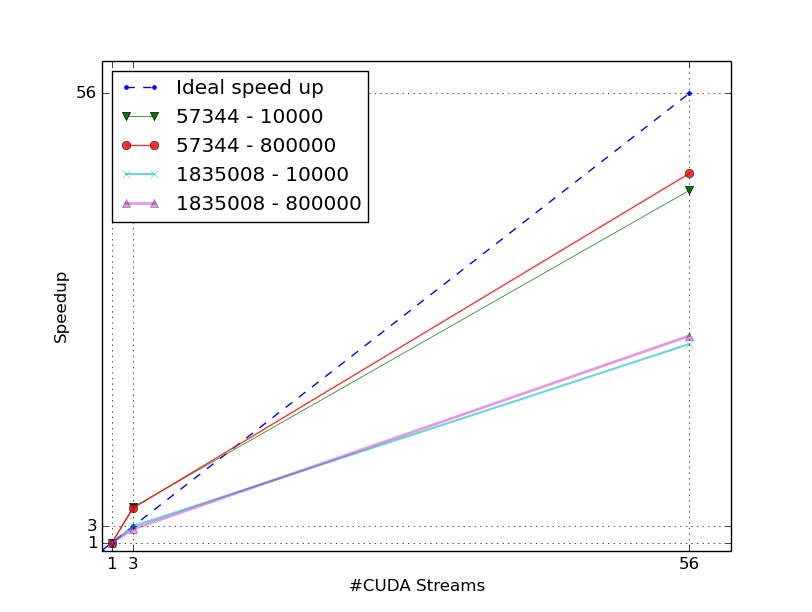
\includegraphics[scale=0.7]{plots/figure_25.png}
		\caption{Speedup for 3 and 56 CUDA streams on P100 device.}
		\label{fig:p100sp}
	%\end{figure}
	% \vspace*{\floatsep}
	%\begin{figure}
		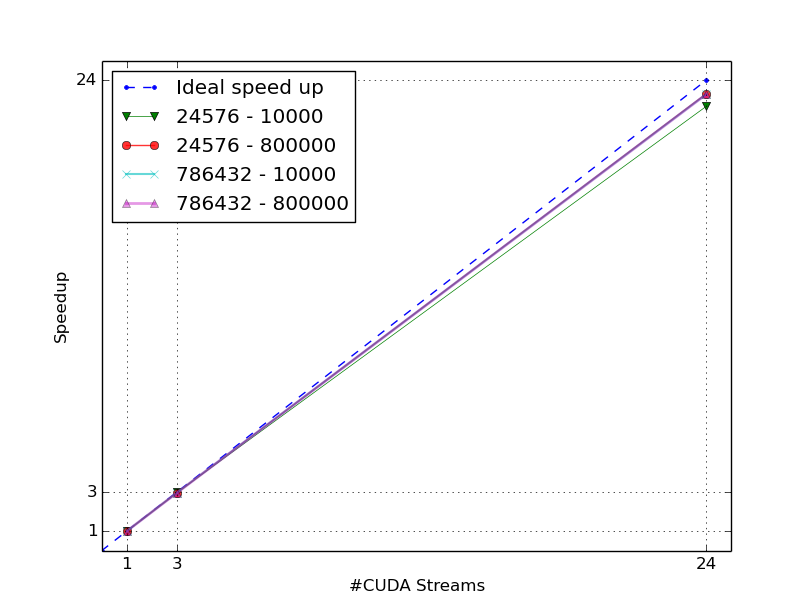
\includegraphics[scale=0.7]{plots/figure_26.png}
		\caption{Speedup for 3 and 56 CUDA streams on M40 device.}
		\label{fig:m40sp}
	\end{figure}
	To have an overall view on speedup we also present plots for both P100, in  \hyperref[fig:p100sp]{Figure 5.1}, and M40, in \hyperref[fig:m40sp]{Figure 5.2}.\\
	The two plots show the speedups only for a part of the real input dataset; in particular, each plot shows the smaller and bigger input stream length and for both it shows the smaller and bigger kernel iterations number.
	
	From the two plots we can clearly see how performances increase proportionally to the number of CUDA streams\footnote{More precisely this gain is bounded to the number of Streaming Multiprocessors the GPU exploits.}.
			
			
	{\large \textbf{Bigger buffers}}\\\\
			All relative measures to 2048 items buffers are reported in Table ***
%\end{enumerate}


%%%%%%%%%%%%%%%%%%%
%%%%% MAT MUL %%%%%
%%%%%%%%%%%%%%%%%%%
\section{Matrix Multiplication}
With Matrix multiplication we're facing a kernel mostly memory-bound, so we had to make some slightly different tests with respect to the ones in simple-computation kernel.\\
Note that, even if the logic is the same as the previous application, there are some details to redefine.\\
First of all, before we were dealing with an input stream of floats that were accumulated in buffers, here we have an input stream of matrices. In particular as soon as we have two available input matrices, they're sent out to device to apply the matrix multiplication kernel. Finally we get back to host with the result matrix, that will be one of the output stream components.

Another assumption is that, for simplicity, we're measuring on square matrices case, even if code was implemented for non-square case too. \\
Thus we performed the following executions:
%BLOCK=32
%matSize=(128 512 1024)
%#nStreams=(0 3 56)
%nMats=(256 1024 2048) # 14680064 29360128)
%dpSize=(2048 3840 5504 7680 8192 15360)

	\begin{table}	
		\centering
		\begin{tabular}{| c | c | c | c |} 
			\hline
			
			 \multicolumn{2}{c}{\textbf{Tesla P100}} & \multicolumn{2}{c}{\textbf{Tesla M40}} \\ [0.5ex]
			 % & \textbf{Tesla P100} & \textbf{Tesla M40} \\ 
			\hline\hline
			
			\textbf{Mat. Order} & \textbf{In stream limit} & \textbf{Mat. Order} & \textbf{In stream limit}  \\ 
			\hline
			128 & 225 & 64 & 100  \\ 
			\hline	
			256 & 441 & 128 & 196  \\ 
			\hline	
			512 & 900 & 256 & 400  \\ 
			\hline		
			1024 & 1764 & 512 & 784  \\ 
			\hline			
			2048 &  & 1024 &  \\
			\hline
			\hline				
			%3 670 016 & ---- & ---- & ---- \\
			%\hline
			
			\multicolumn{2}{c}{Data Parallel} &  \multicolumn{2}{c}{Data Parallel} \\ [0.5ex]
			% & \textbf{Data Parallel} & \textbf{Data Parallel} \\ 
			\hline\hline
			\multicolumn{2}{c}{1920} & \multicolumn{2}{c}{1280} \\ [0.5ex]
			% & \textbf{Data Parallel} & \textbf{Data Parallel} \\ 
			\hline			
			\multicolumn{2}{c}{2816} & \multicolumn{2}{c}{1792} \\ [0.5ex]
			\hline
			\multicolumn{2}{c}{3840} & \multicolumn{2}{c}{2560} \\ [0.5ex]
			\hline
			\multicolumn{2}{c}{5632} & \multicolumn{2}{c}{3584} \\ [0.5ex]
			\hline
			\multicolumn{2}{c}{7680} & \multicolumn{2}{c}{5120} \\ [0.5ex]
			\hline
			\multicolumn{2}{c}{11264} & \multicolumn{2}{c}{7168} \\ [0.5ex]
			\hline

		\end{tabular}
		\caption{Input dataset for Matrix Multiplication kernel. Above Stream parallel configuration, below Data Parallel correspondent.}	
		\label{tab:matdata}		
	\end{table}
	
\begin{enumerate}
	\item \textbf{Classic data parallel approach}
	As always we have to put a limit on input stream, so that we can measure completion times and compare different approaches.\\
	To test the data parallel version it suffices to treat input/output streams as huge matrices.
	This means that we'll do computations, no longer on stream of small data structures, but on a unique big data structure.\\
	So, for example:
	\begin{itemize}
		\item We have two input streams, each has limit to 9 square matrices of order 2 (one input stream is for \textbf{A} matrices and one for \textbf{B});
		\item So suppose that our stream parallel model, sends out one matrix A and one B at time;
		\item Then we launch the kernel, performing the matrix multiplication, this will give back a matrix result C;
		\item This means in total we will perform 9 multiplications between couples of matrices, giving 9 result matrices;
		\item If we consider those 9 small matrices as block matrices, we can combine them into a bigger one;
		\item This will be equivalent to pick A and B matrices each of order 6;
		\item note that, for simplicity, we'll choose as input stream limit a square number, so that the equivalent combined data structure will be again square;
		\item In our example 9 is a square number so that we can obtain as composed matrix dimension \([(2\cdot3)\times(2\cdot3)] = [6\times6]\)  
	\end{itemize} 
	In \hyperref[tab:matdata]{Table 5.2}, in the lower portion, are showed the matrices orders we used to test data parallel version for matrix multiplication. 
	By giving these values as (square) matrix dimension and computing only one multiplication between matrices, we'll get the relative comparison to some Stream parallel versions \footnote{We'll see later what cases we match between data and stream parallel to make comparisons.}.
	
	\item \textbf{Streaming parallel}
	As we mentioned before, we have to put a limit on the stream length for both streams of input matrices.\\
	In the upper portion of \hyperref[tab:matdata]{Table 5.2} are reported all input stream limit, for each of them we test all of matrices order.\\
	For every combination given by the input dimensions, we'll test for different numbers of CUDA streams: \textbf{Zero}, \textbf{Three} and \textbf{N\textsubscript{SM}} CUDA Streams (with \(N_{SM} \ =\# Streaming \ Multiprocessors\)).
	The above test on different numbers of non-default streams, is implemented in a totally analogous way to the one for Simple-computation Kernel. And the reasons why we test for those numbers of streams are the same too.
\end{enumerate}



\subsection{Results}
\begin{table}	
	\centering
	\begin{tabular}{ | c c c  | c c c | } 
		\hline
		\multicolumn{3}{c}{\textbf{Tesla P100 (zero Streams)}} & \multicolumn{3}{c}{\textbf{Tesla M40 (zero Streams)}}\\ [0.5ex]
		% & \textbf{Tesla P100} & \textbf{Tesla M40} \\ 
		\hline\hline
		Event Times  & Number of Mats & Mat. Order & Event Times  & Number of Mats & Mat. Order  \\
		\hline
		
		
		86.8854&	225&	\multirow{4}{*}{128}&	17.4869&	100&	\multirow{4}{*}{64}\\
		175.189&	441&	&	34.8778&	196&	\\
		359.9716&	900&	&	70.9718&	400&	\\
		725.5573&	1764&	&	139.3896&	784&	\\
		\hline
		334.0376&	225&	\multirow{4}{*}{256}&	36.2095&	100&	\multirow{4}{*}{128}\\
		672.9463&	441&	&	74.2685&	196&	\\
		1435&	900&	&	147.7336&	400&	\\
		2828.5366&	1764&	&	299.138&	784&	\\
		\hline
		1673.2133&	225&	\multirow{4}{*}{512}&	186.3913&	100&	\multirow{4}{*}{256}\\
		3325.6533&	441&	&	368.6813&	196&	\\
		6611.7566&	900&	&	786.7536&	400&	\\
		12919.6666&	1764&	&	1603.4933&	784& \\
		\hline
		10998.7666&	225&	\multirow{4}{*}{1024}&	1256.4&	100&	\multirow{4}{*}{512}\\
		21511.1666&	441&	&	2479.4333&	196&	\\
		43828.7666&	900&	&	5162.6333&	400&	\\
		85853.0333&	1764&	&	9791.98&	784&	\\
		\hline
		80764.8666&	225&	\multirow{4}{*}{2048}&	9075.22&	100&	\multirow{4}{*}{1024}\\
		158136.3333& 441&	&	17849.5666&	196&	\\
		309724.6666& 900&	&	36441.3666&	400&	\\
		604324&	1764&	&	72396.8666&	784&	\\
		
		\hline
		
	\end{tabular}
	\caption{Device completion times for Mat-Mul kernel, without using CUDA Streams (zero streams), results are reported for both P100 and M40.}	
	\label{tab:matvgszero}		
\end{table}

\begin{table}	
	\centering
	\begin{tabular}{ | c c c  | c c c | } 
		\hline
		\multicolumn{3}{c}{\textbf{Tesla P100 (zero Streams)}} & \multicolumn{3}{c}{\textbf{Tesla M40 (zero Streams)}}\\ [0.5ex]
		% & \textbf{Tesla P100} & \textbf{Tesla M40} \\ 
		\hline\hline
		Event Times  & Number of Mats & Mat. Order & Event Times  & Number of Mats & Mat. Order  \\
		\hline

		25.5549& 225&	\multirow{4}{*}{128}&	5.2046&	100&	\multirow{4}{*}{64}\\
		53.2203&	441&	&	10.7422&	196&	\\
		102.0575&	900&	&	23.9773&	400&	\\
		193.2436&	1764&	&	47.1808&	784&	\\
		\hline
		148.1446&	225&	\multirow{4}{*}{256}&	21.5294&	100&	\multirow{4}{*}{128}\\
		289.6773&	441&	&	41.9395&	196&	\\
		590.6776&	900&	&	74.5879&	400&	\\
		1157&	1764&	&	143.3123&	784&	\\
		\hline
		1173.3466&	225&	\multirow{4}{*}{512}&	129.985&	100&	\multirow{4}{*}{256}\\
		2298.3866&	441&	&	254.2516&	196&	\\
		4690.97&	900&	&	518.3303&	400&	\\
		9205.5&	1764&	&	1016.28&	784&	\\
		\hline
		9371.7766&	225&	\multirow{4}{*}{1024}&	1033.9166&	100&	\multirow{4}{*}{512}\\
		18371.2666&	441&	&	2027.17&	196&	\\
		37480.4&	900&	&	4136.54&	400&	\\
		73258.6666&	1764&	&	8113.0933&	784&	\\
		\hline
		74966.4666&	225&	\multirow{4}{*}{2048}&	8273.1066&	100&	\multirow{4}{*}{1024}\\
		146156.3333&	441&	&	16194.1&	196&	\\
		285788.3333&	900&	&	33041.1&	400&	\\
		559469.6666&	1764&	&	64763.6666&	784&	\\
		
		\hline
		
		
	\end{tabular}
	\caption{Device completion times for Mat-Mul kernel, with three CUDA Streams, results are reported for both P100 and M40.}	
	\label{tab:matvgsThree}		
\end{table}


\begin{table}	
	\centering
	\begin{tabular}{ | c c c  | c c c | } 
		\hline
		\multicolumn{3}{c}{\textbf{Tesla P100 (zero Streams)}} & \multicolumn{3}{c}{\textbf{Tesla M40 (zero Streams)}}\\ [0.5ex]
		% & \textbf{Tesla P100} & \textbf{Tesla M40} \\ 
		\hline\hline
		Event Times  & Number of Mats & Mat. Order & Event Times  & Number of Mats & Mat. Order  \\
		\hline
		
		
		%86.8854&	225&	\multirow{4}{*}{128}&	17.4869666667&	100&	64\\
		20.8758&	225&	\multirow{4}{*}{128}&	2.739&	100&	\multirow{4}{*}{64}\\
		40.5783&	441&	&	5.0942&	196&	\\
		74.6636&	900&	&	10.0277&	400& \\
		145.4766&	1764&	&	19.8252&	784&	\\
		\hline
		147.765&	225& \multirow{4}{*}{256}&	19.3538&	100&	\multirow{4}{*}{128}\\
		288.5343&	441&	&	37.8560&	196&	\\
		588.9643&	900&	&	65.6809&	400&	\\
		1153.7333&	1764&	&	128.317&	784&	\\
		\hline
		1173.32&	225&\multirow{4}{*}{512}&	130.0533&	100&	\multirow{4}{*}{256}\\
		2298.3966&	441&	&	254.281&	196&	\\
		4690.9633&	900&	&	518.615&	400&	\\
		9202.3333&	1764&	&	1016.55&	784&	\\
		\hline
		9371.0433&	225&	\multirow{4}{*}{1024}&	1034.0666&	100&	\multirow{4}{*}{512}\\
		18374.7&	441&	&	2027.2866&	196&	\\
		37474.7&	900&	&	4136.7066&	400&	\\
		73348.3333&	1764&	&	8110.9966&	784&	\\
		\hline
		74971.6666&	225&	\multirow{4}{*}{2048}&	8262.7533&	100&	\multirow{4}{*}{1024}\\
		146175.6666&	441&	&	16202.4666&	196&	\\
		285955.6666&	900&	&	33059.2666&	400&	\\
		559425&	1764&	&	64786.5333&	784&	\\
		
		\hline
		
		
	\end{tabular}
	\caption{Device completion times for Mat-Mul kernel, with as many CUDA Streams as SM number, results are reported for both P100 and M40.}	
	\label{tab:matvgsSM}		
\end{table}






All the above tests on Matrix Multiplication Kernel give us the measures of device times.\\
Below we'll see that completion times and performance will notably be different, with respect to the previous computation-bound application.

All collected elapsed times are reported in \hyperref[tab:matvgszero]{Table 5.6}, for the zero-streams version, in \hyperref[tab:matvgsThree]{Table 5.7}, for the three-streams one, and \hyperref[tab:matvgsSM]{Table 5.8}, for the SM-streams version.\\
From these tables we can highlight some behaviors:
\begin{itemize}
	\item input streams of matrices have lengths that grow by a factor of 2 and it's easy to see that this makes a proportional increase in completion times, ie even measures grows by factors of 2;
	
	\item input matrix sizes again grow of 2x each, but in this case the completion times don't grow proportionally;
	
	\item for zero-streams we can see that, as the matrix order grows by a factor of 2, the completion time can increase from \~4x to \~7x; 
	
	\item for three-streams we can see that, as the matrix order grows by 2x, the completion time can increase from \~5x to \~7.9x; 
	
	\item finally for SM-streams we can see that, the completion time can increase from \~7x to \~8x.
\end{itemize}
Those evidences holds for both machines measures and they give some hints on matrix multiplication behavior.\\
The first point tells us that elapsed time to send/receive to/from the device grows linearly with the number of matrices, so this input variable would not affect performances. Especially, no matter the CUDA streams amount we decide to use, the increase by 2x of matrices quantity, will always give a growth of 2x in measures.

The other points tells us that, as matrix order increases, we'll get worser and worser performances. Clearly this doesn't depend on CPU/GPU data transfers overhead \footnote{Host/device transfers, in general, give a bigger overhead when lot of calls are issued.}, otherwise we'd have the same behavior when number of matrices grows.\\
So, the cause must reside exclusively on what happens inside the GPU. In reality, the classic matrix multiplication is a well known problem in GPUs paradigm and it's also known as a not-so-efficient problem. \\
This is because, the simpler implementation, at each iteration, performs more \textit{global memory}/\textit{registers} transfers than effective calculations. So that's why this kind of matrix multiplication is considered memory-bound.\\
So, the more elements a matrices have, the more data transfers (internal to the device) the GPU will have to perform and the more active threads will stall waiting for data to be available for computations.\\

\begin{table}	
	\centering
	\begin{tabular}{ | c | c | c | c  || c | c | c | c | } 
		\hline
		\multicolumn{4}{c}{\textbf{Tesla P100 (56 Streams)}} & \multicolumn{4}{c}{\textbf{Tesla M40 (24 Streams)}}\\ [0.5ex]
		% & \textbf{Tesla P100} & \textbf{Tesla M40} \\ 
		\hline\hline
		\textbf{Mat. Number}  & \textbf{Mat. Order} & \textbf{Sp(3)} & \textbf{Sp(56)} & \textbf{Mat. Number}  & \textbf{Mat. Order}  & \textbf{Sp(3)} & \textbf{Sp(24)} \\
		\hline
		
		
		225& \multirow{4}{*}{128}&	3.3999&	4.1620&	100&	\multirow{4}{*}{64}&	3.3598&	6.3839\\
		441& &	3.2917&	4.3173&	196&	&	3.2467&	6.8464\\
		900& &	3.5271&	4.8212&	400&	&	2.9599&	7.0775\\
		1764& &	3.7546&	4.9874&	784&	&	2.9543&	7.0309\\
		\hline
		225& \multirow{4}{*}{256}&	2.2548&	2.2606&	100& \multirow{4}{*}{128}& 1.6818&	1.8709\\
		441& & 2.3230&	2.3322&	196& & 1.7708& 1.9618\\
		900& & 2.4294&	2.4364&	400& & 1.9806&	2.2492\\
		1764& &	2.4447&	2.4516&	784& & 2.0873&	2.3312\\
		\hline
		225& \multirow{4}{*}{512}&	1.4260&	1.4260&	100& \multirow{4}{*}{256}&	1.4339&	1.4331\\
		441& &	1.4469&	1.4469&	196&  & 1.4500&	1.4498\\
		900& &	1.4094&	1.4094&	400& &	1.5178&	1.5170\\
		1764& &	1.4034&	1.4039&	784& &	1.5778&	1.5773\\
		\hline
		225& \multirow{4}{*}{1024}&	1.1736&	1.1736&	100&	\multirow{4}{*}{512}&	1.2151&	1.2150\\
		441& &	1.1709&	1.1706&	196& & 1.2231&	1.2230\\
		900& &	1.1693&	1.1695&	400& &	1.2480&	1.2480\\
		1764& &	1.1719&	1.1704&	784& &	1.2069&	1.2072\\
		\hline
		225& \multirow{4}{*}{2048}&	1.0773&	1.0772&	100&	\multirow{4}{*}{1024}&	1.0969&	1.0983\\
		441& &	1.0819&	1.0818&	196& &	1.1022&	1.1016\\
		900& &	1.0837&	1.0831&	400& &	1.1029&	1.1023\\
		1764& &	1.0801&	1.0802&	784& &	1.1178&	1.1174\\
		
		\hline
		
		
	\end{tabular}
	\caption{Here are showed speedups for all data sets of simple-computation kernel. Results are reported for both devices.}	
	\label{tab:matspeedup}		
\end{table}
So we'll now focus on speedups, to see that this memory-bound behavior will be reflected on our GPU Farm approach. All speedups are listed in \hyperref[tab:matspeedup]{Table 5.9}.\\
From those results, we can mainly observe that:
\begin{itemize}
	\item \textit{Sp(3)} gives results near to the expected value, ie \~3 for the smaller matrix sizes (128-256 for the P100, 64 for the M40);
	
	\item 	\textit{Sp(SM)} gives a really poor gain w.r.t. \textit{Sp(3)};
	
	\item all speedups degrade  to \~1 as the matrix order grows.
\end{itemize}




%\begin{figure}
%	\vspace{-1.5cm}
%	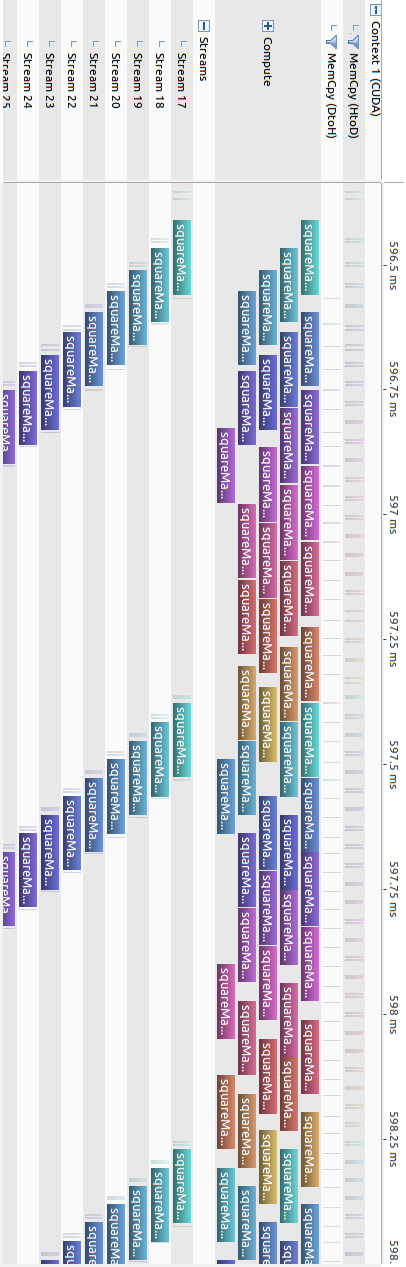
\includegraphics[scale=0.7]{plots/matmul784_64_timeline.png}
%	\caption{NVIDIA Visual profiler generated \textit{timeline} on M40, using 24 CUDA streams and running code for 784 matrices of size 64.}
%	\label{fig:mat64timeln}
%\end{figure}

% \vspace*{\floatsep}
%\begin{figure}
%	\vspace{-1.5cm}
%	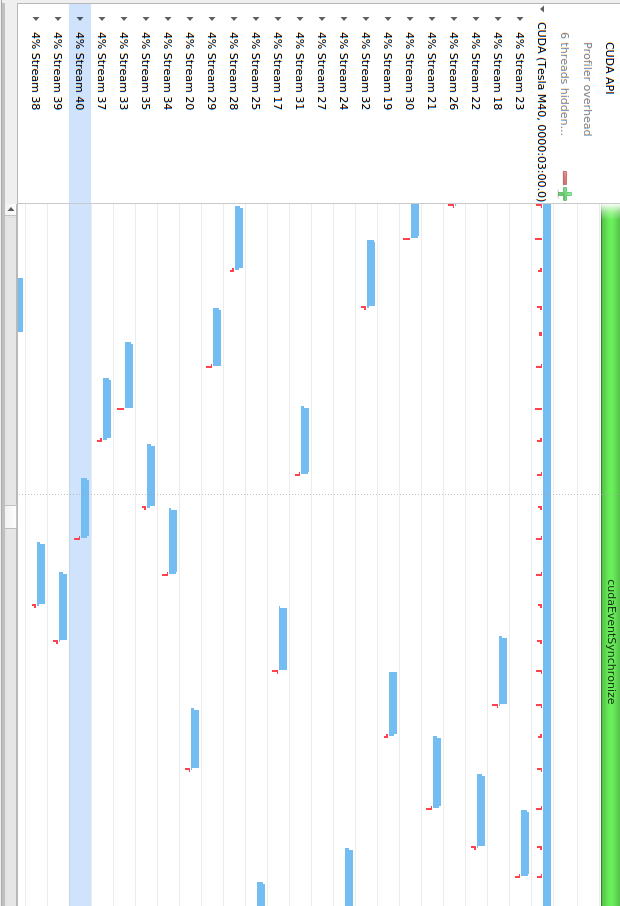
\includegraphics[scale=0.7]{plots/mat_big_str_nsight.png}
%	\caption{Nsight profiler execution on M40, using 24 CUDA streams and running code for 784 matrices of size 256.}
%	\label{fig:matnsightbig}
%\end{figure}

%\begin{figure}[!tbp]
%	\centering
%	\vspace{-1.5cm}
%	\begin{minipage}[b]{0.1\textwidth}
%		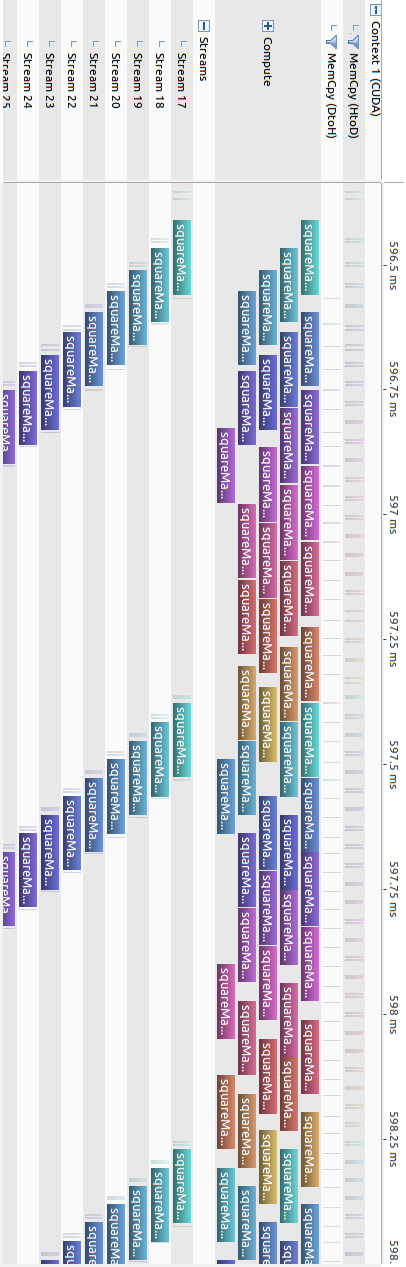
\includegraphics[scale=0.5]{plots/matmul784_64_timeline.png}
%		\caption{NVIDIA Visual profiler generated \textit{timeline} on M40, using 24 CUDA streams and running code for 784 matrices of size 64.}
%		\label{fig:mat64timeln}
%	\end{minipage}
	
	%\vfill
%	\begin{minipage}[b]{0.4\textwidth}
%		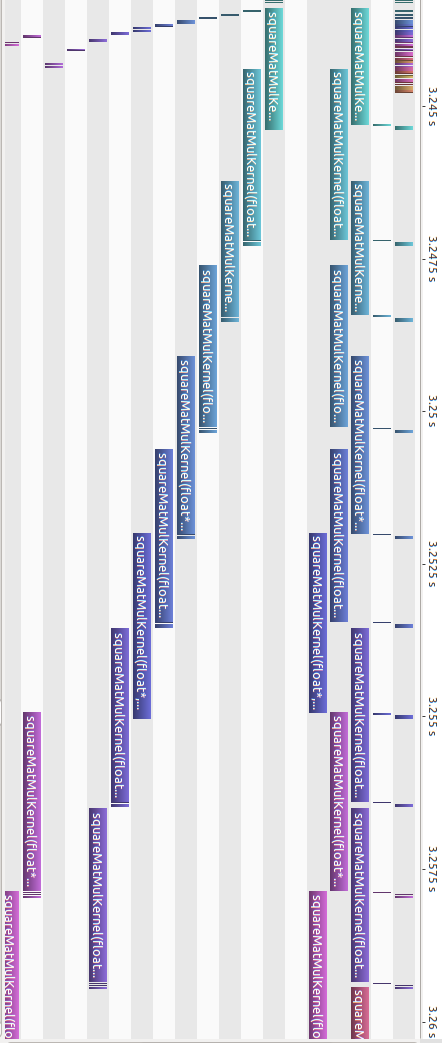
\includegraphics[scale=0.5]{plots/matmul784_256_timeline.png}
		%\caption{Same,except for matrices size set to 256.}
		%\label{fig:mat256timeln}
%	\end{minipage}
	%\hfill
%	\begin{minipage}[b]{0.4\textwidth}
%		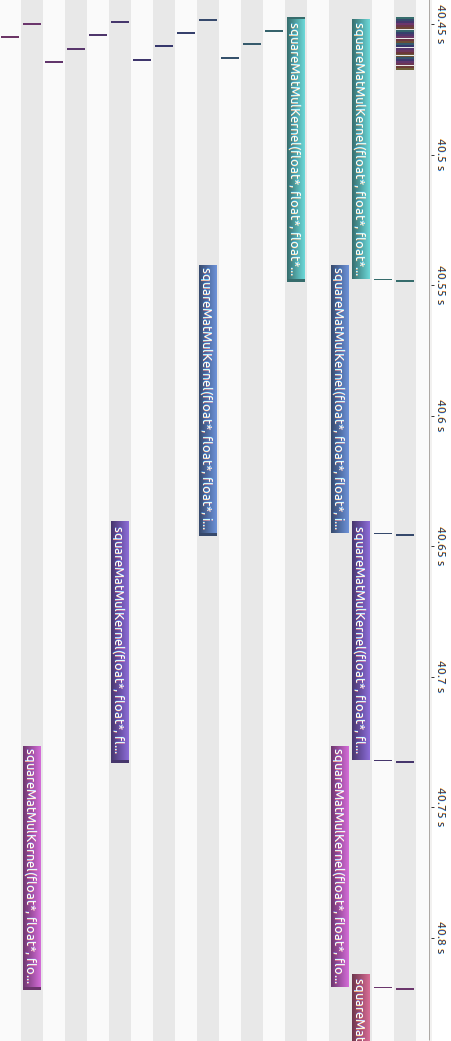
\includegraphics[scale=0.5]{plots/matmul784_1024_timeline.png}
		%\caption{Same,except for matrices size set to 1024.}
		%\label{fig:mat1024timeln}
%	\end{minipage}
	
%\end{figure}



%\begin{figure}[!tbp]
%	\centering
%	\vspace{-1cm}
	%\raggedright
%	\subfloat[Matrix size 64]{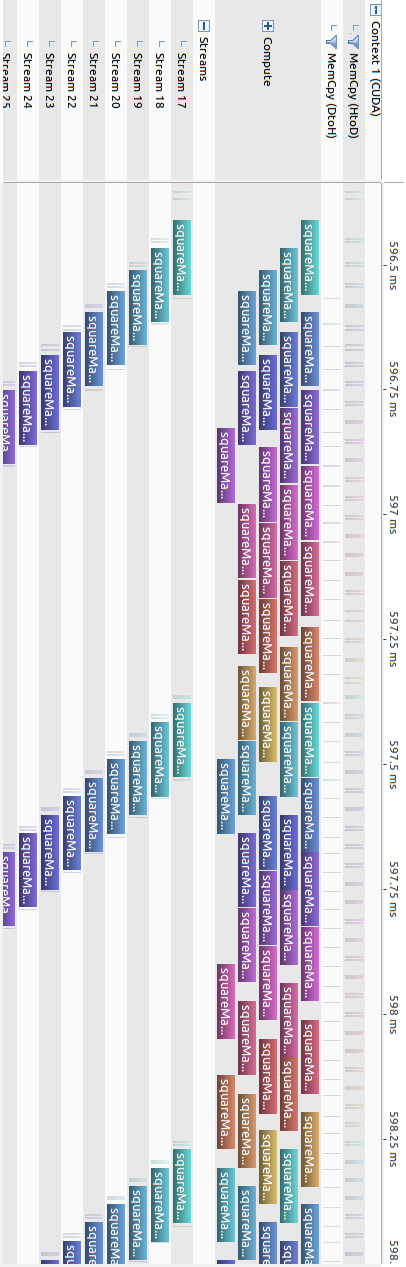
\includegraphics[width=0.4\textwidth]{plots/matmul784_64_timeline.png}\label{fig:timeln64}}
%	\raggedleft
%	\hfill
%	\subfloat[Matrix size 256]{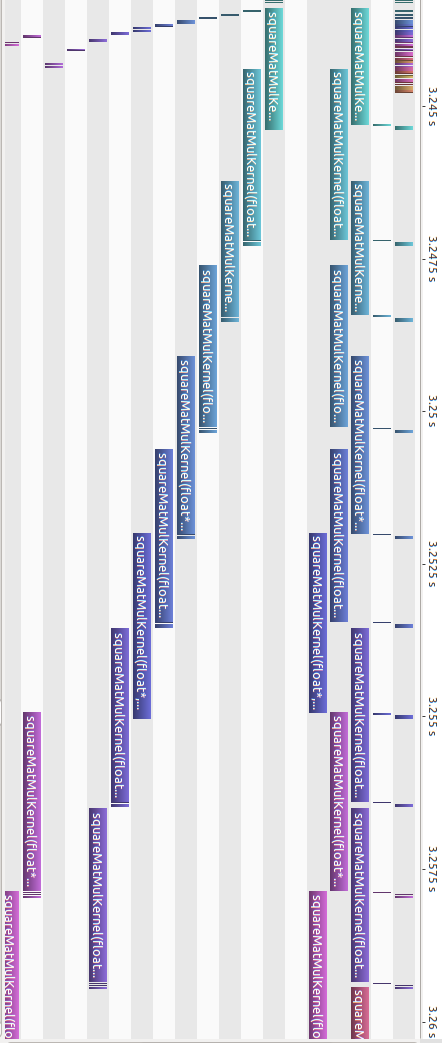
\includegraphics[width=0.2\textwidth]{plots/matmul784_256_timeline.png}\label{fig:timeln256}}
%	\vfill
%	\subfloat[Matrix size 1024]{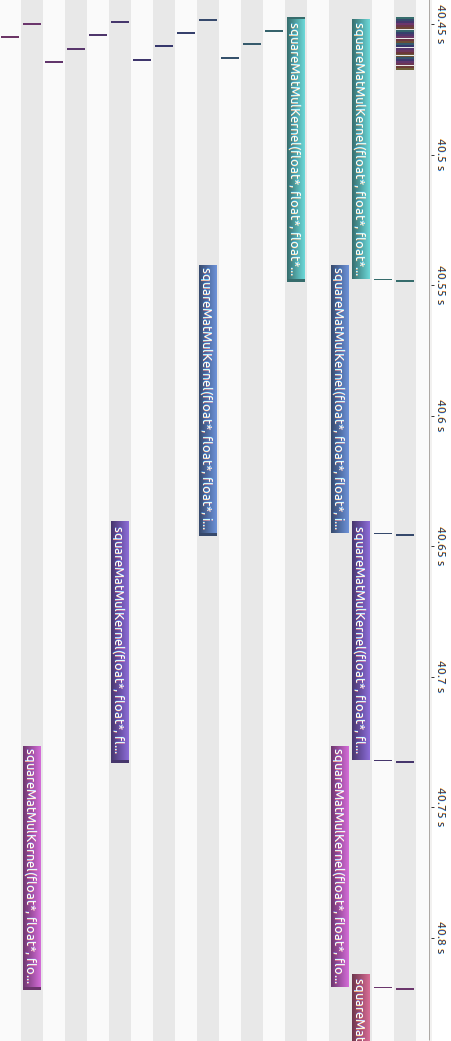
\includegraphics[width=0.2\textwidth]{plots/matmul784_1024_timeline.png}\label{fig:timeln1024}}
%	\caption{NVIDIA Visual profiler generated \textit{timeline} on M40, using 24 CUDA streams and running code for 784 matrices.}
%\end{figure}

\begin{figure}[!tbp]
	\centering
	\vspace{-1cm}
	\hspace{2cm}
	\begin{tabular}[c]{cc}
		\makecell[tl]{\subfloat[Matrix size 256]{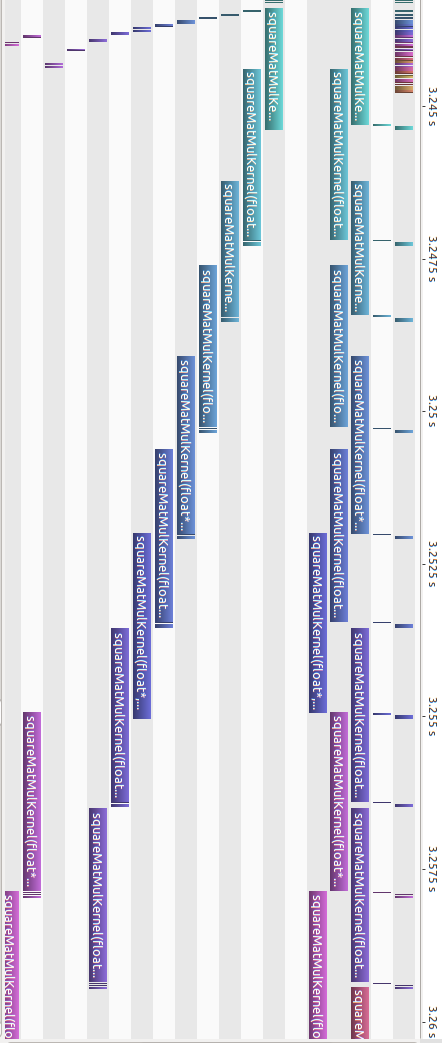
\includegraphics[width=0.32\textwidth]{plots/matmul784_256_timeline.png}\label{fig:timeln256}} \\
		\subfloat[Matrix size 1024]{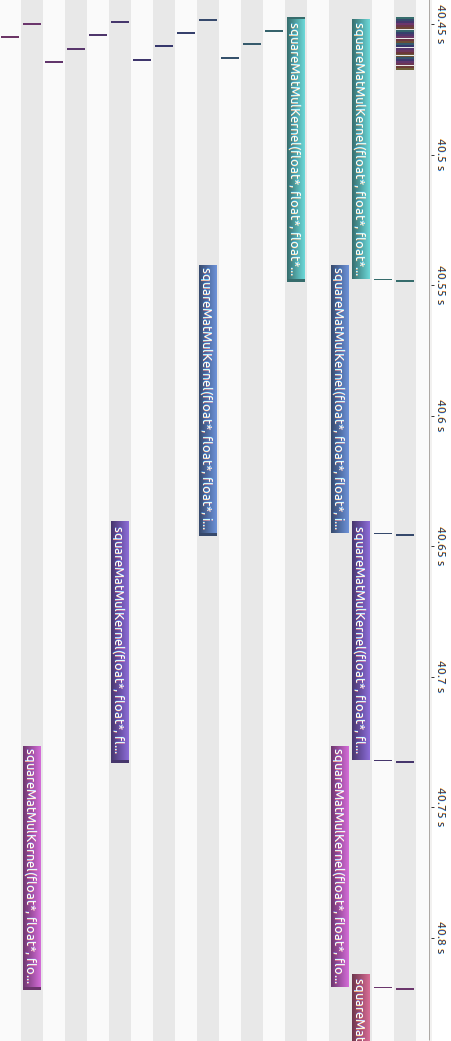
\includegraphics[width=0.32\textwidth]{plots/matmul784_1024_timeline.png}\label{fig:timeln1024}}}
		& \vspace*{2cm}
		\subfloat[Matrix size 64]{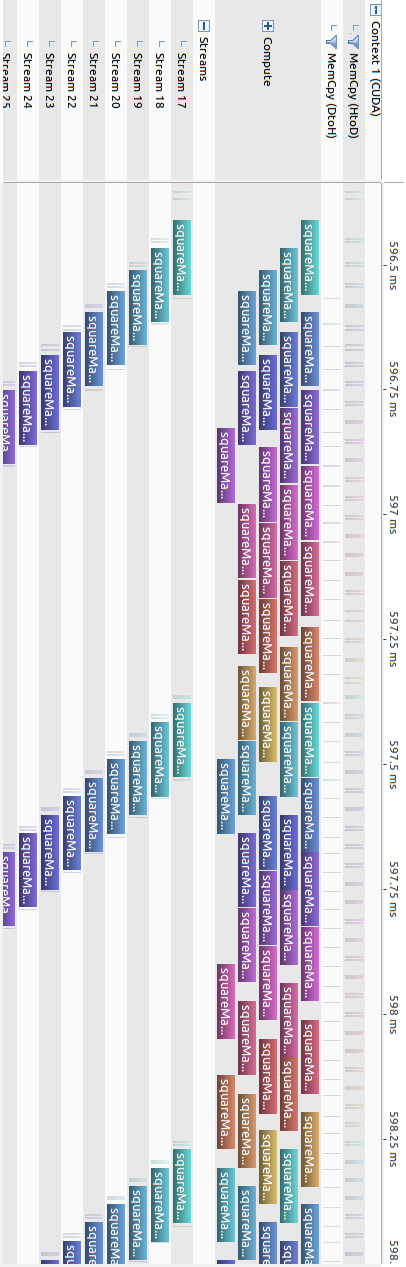
\includegraphics[width=0.45\textwidth]{plots/matmul784_64_timeline.png}\label{fig:timeln64}}\\
		
	%	\subfloat[Matrix size 1024]{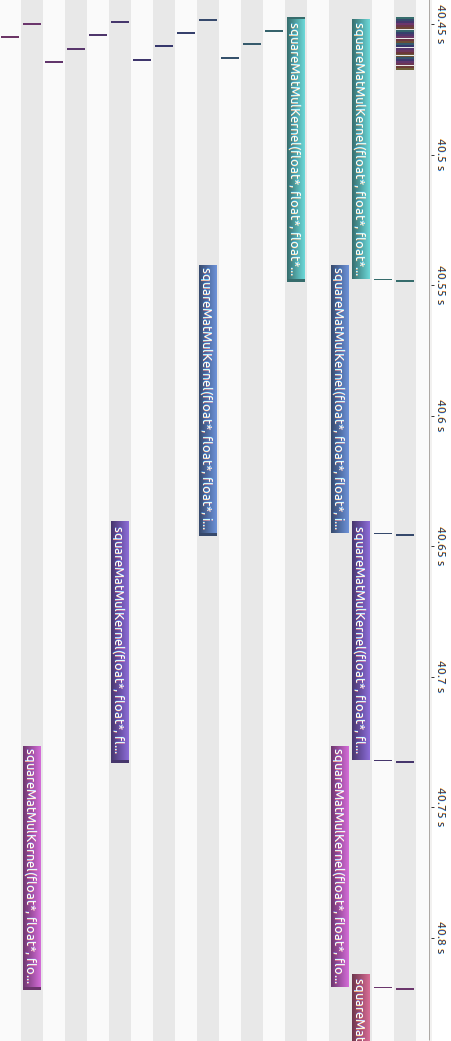
\includegraphics[width=0.2\textwidth]{plots/matmul784_1024_timeline.png}\label{fig:timeln1024}} &\vspace*{1cm} \\
	\end{tabular}    
	\caption{NVIDIA Visual profiler generated \textit{timeline} on M40, using 24 CUDA streams and running code for 784 matrices.}
	\label{fig:timeln}
\end{figure}

This behavior translates in the following: when the matrices get bigger, even if CUDA Streams push to have more simultaneous mat-mul, we'll have a lot of active threads (and so Multiprocessors) busy and probably mainly stalled on gathering floats from global memory.\\
This, in fact, inevitably leads to a very limited amount of gain, even when using a lot of CUDA streams. Furthermore, those results tells us that we will fit in Multiprocessor less matrix multiplication than we expect \footnote{Clearly this holds strictly for the type of matrix multiplication we implemented.}.\\
Profiling the application for some key data set we can inspect the above described facts and the relative reasons.

\begin{figure}[!tb]
	\centering
	\vspace{-2cm}
	%\hspace{2cm}
	\begin{tabular}[c]{cc}
		\multicolumn{2}{c}{\subfloat[Matrix size 64]{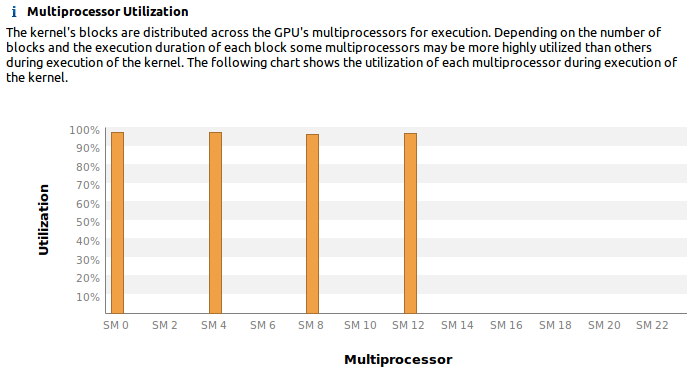
\includegraphics[width=\textwidth]{plots/matmul784_64_SMuse.png}\label{fig:SMuse64}}} \\
		
		\subfloat[Matrix size 1024]{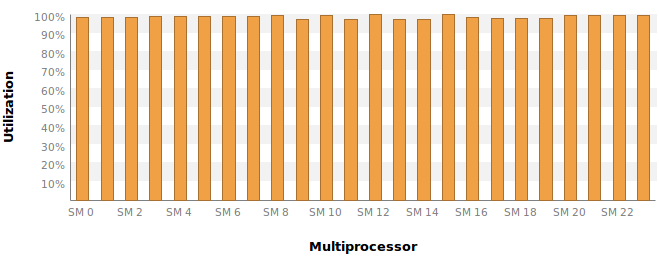
\includegraphics[width=0.5\textwidth]{plots/matmul784_1024_SMuse.png}\label{fig:SMuse1024}}
		&
		\subfloat[Matrix size 256]{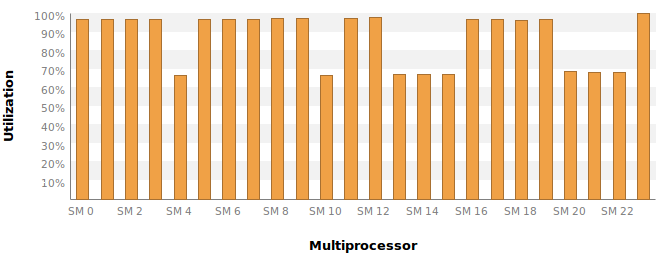
\includegraphics[width=0.5\textwidth]{plots/matmul784_256_SMuse.png}\label{fig:SMuse256}}\\
		
		%	\subfloat[Matrix size 1024]{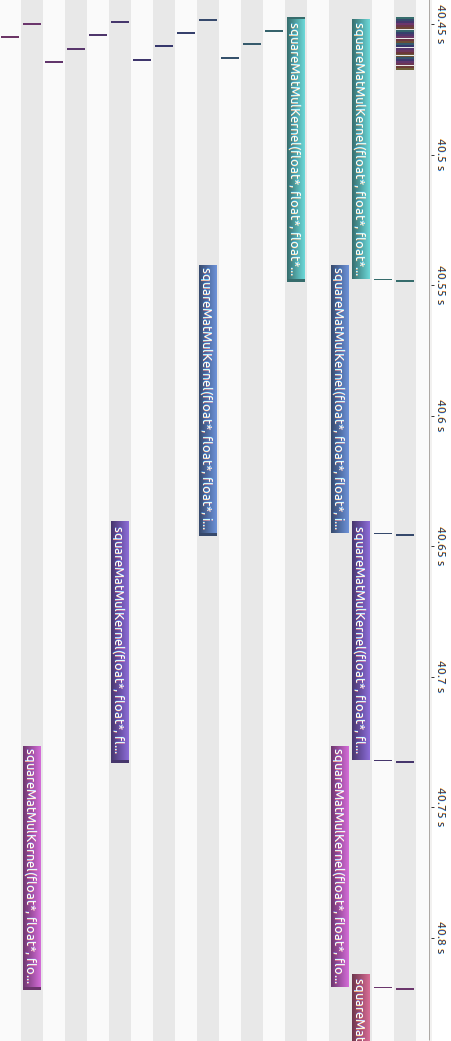
\includegraphics[width=0.2\textwidth]{plots/matmul784_1024_timeline.png}\label{fig:timeln1024}} &\vspace*{1cm} \\
	\end{tabular}    
	\caption{NVIDIA Visual profiler generated \textit{timeline} on M40, using 24 CUDA streams and running code for 784 matrices.}
	\label{fig:SMuse}
\end{figure}

In \hyperref[fig:timeln]{Figure 5.3} we can have a visual cue on what is happening during an execution of mat-mul on M40, with 24 CUDA streams, having an input stream of 784 matrices of sizes: 64x64 (\hyperref[fig:timeln64]{Figure 5.3}), 256x256(\hyperref[fig:timeln256]{Figure 5.3}), 1024x1024(\hyperref[fig:timeln1024]{Figure 5.3}).\\
%In this screen shot on top there's the timeline of all CUDA APIs that have been called, under that we find a light blue line representing all kernel activities in M40 and attached below there are lot of red ticks that shows all memory copy activities (from host to device and viceversa).\\
Analyzing the figure we can see that the amount of overlapping between operations in different streams is quite limited in general, this just confirms what we saw from speedups.\\
From the above pictures, we can observe that in 64-sized case we're having a slightly better overlapping and a little more kernels running at the same time. In this case this may happens for few reasons:
\begin{itemize}
	\item grid and block sizes are smaller for each kernel launch, so this allow to have multiple kernels fit in SMs;
	\item kernel durations are shorter so this gives a further chance to overlap data transfers, other than kernel.
\end{itemize} 

A 64x64 result matrix (say C) is managed by a grid of 2x2 blocks, each of which has 32x32 threads\footnote{This depends on how we implemented kernel launch, that is the classical kernel launch approach setting blocks at the maximum size possible. Remember implementations in \hyperref[chap:impl]{Chapter 4}}, while a 256x256 C is managed by a grid of 8x8 blocks, each of which having 32x32 threads and, finally, a 1024x1024 C is managed by a grid of 32x32 blocks, each of which having 32x32 threads.\\
This means that, in the two latter cases, we don't even have all blocks of a kernel launch fitting in all the SMs. If this may theoretically give a full occupancy of the GPU by a certain kernel, from the other side means saturate the cores without permitting other launches to fit, until the residing kernels ends or, at least, some resources are available.

We can confirm this fact by looking at the occupancy graphs (generated from Visual Profiler), showed in \hyperref[fig:SMuse]{Figure 5.4}. In 64-sized case we've only 4 SMs almost fully employed, while in the other cases all SMs are almost busy.\\
The above cases exposes an example of the fact that \textit{not always a high or full occupancy may give better performances} \cite{loweroccupancy,cudabestpractices}, it strongly depends on the kernel nature.\\
On the other side as we decrease the matrices size we can't exploit enough resources. As we can see from \hyperref[fig:timeln64]{Figure 5.3} we have a better overlapping, but it seems that kernels lasts too little, so the host can't push kernels quickly enough to fill SMs. In fact Visual Profiler suggests us that those kernels perform a really poor amount of computations, especially with respect to memory latencies, see figure \hyperref[fig:mat62latency]{Figure 5.5}.\\ 
\begin{figure}[!tb]
	%\centering
	\vspace{-1cm}
	\hspace{-1cm}
	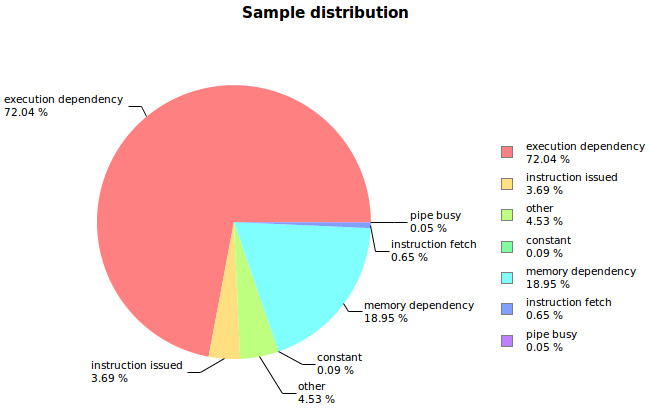
\includegraphics[scale=0.8]{plots/matmul784_64_kerlatencies.png}
	\caption{Nsight profiler execution on M40, 24 CUDA streams, 784 matrices of size 256. This graph gives the types and relative amounts of latencies inside our mat-mul kernel code.}
	\label{fig:mat62latency}
\end{figure}
This pie chart shows that most of the time kernels is idle on:
\begin{itemize}
	\item execution dependency\footnote{Execution dependency stall can be potentially reduced by increasing instruction-level parallelism Instruction-Level Parallelism, a.k.a. ILP, means that we can improve parallelism by increasing the amount of instructions for each thread. This can translate in less threads having a greater work-load each. }, ie an input required by the issued instruction isn't yet available; 
	
	\item memory dependency\footnote{ Memory dependency stall type can potentially be reduced by optimizing memory alignment and access patterns}, a load/store cannot be made because the required resources aren't available or are fully utilized, or too many requests of a given type are outstanding.
\end{itemize}
This demonstrates the fact that matrix multiplication is a memory-bound problem in GPU and, so,poor in computation amount.\\
This is why we have really short kernels for small input data size and heavy kernels for bigger input sizes.


%%%%%%%%%%%%%%%%%%%%%%
%%%%% IMAGE PROC %%%%%
%%%%%%%%%%%%%%%%%%%%%%
\section{Image processing}
With image processing, ie Blur Box algorithm we're facing a kernel mostly memory-bound and especially rich of divergent execution flows, so we made similar tests to the ones for Matrix multiplication.\\
Thus we performed the following executions:
%BLOCK=1024
%imgSize=(128 256)
%#nStreams=(0 3 56)
%nImgs=(256 1024) # 14680064 29360128)
%dpSize=(4096 8192)


\begin{table}	
	\centering
	\begin{tabular}{| c | c |} 
		\hline
		
		 \multicolumn{2}{c}{\textbf{Tesla P100} \& \textbf{Tesla M40}} \\ [0.5ex]
		%& \textbf{Tesla P100} & \textbf{Tesla M40} \\ 
		\hline\hline
		
		\textbf{Img. Order} & \textbf{In stream limit} \\ 
		\hline
		128 & 64 \\ 
		\hline		
		256	& 256 \\ 
		\hline			
		512	& 1024 \\ 
		\hline	
		\hline
			

	\multicolumn{2}{c}{\textbf{Data Parallel Tesla P100 \& Tesla M40}} \\ [0.5ex] 
		\hline\hline		
		\multicolumn{2}{c}{1024 \((=128\cdot8)\)} \\ [0.5ex] 
		
		
		
		\multicolumn{2}{c}{2048 \((=128\cdot32)\)} \\ [0.5ex] 
		
		\multicolumn{2}{c}{4096 \((=128\cdot32)\)} \\ [0.5ex] 
		
		\multicolumn{2}{c}{8192 \((=256\cdot32)\)} \\ [0.5ex] 
		\hline
		
		
	\end{tabular}
	\caption{Input dataset for Image Processing kernel. Above Stream parallel configuration, below Data Parallel correspondent.}	
	\label{tab:imgdata}		
\end{table}

\begin{enumerate}
	\item \textbf{Classic data parallel approach}
	If we think to a picture as a matrix of pixels, then it's easy to see the analogy to the previous application.\\
	In particular the Data Parallel approach will be tested giving an image of large dimensions, instead of a stream of small images.\\
	Again we can consider a single big image, as formed by merging smaller ones. Similarly to matrix multiplication case we chose, as input stream limits, square numbers to make possible a balanced comparison to the correspondent square picture in data parallel.\\
	In the lower part of \hyperref[tab:imgdata]{Table 5.3} we show the order of dimension of the images used to compare to some streaming parallel cases.
	
	\item \textbf{Streaming parallel}
	
	As previous cases of Farm parallel pattern, we have to put a limit on the stream length for input stream of images.\\
	In the upper portion of \hyperref[tab:imgdata]{Table 5.3} are reported input stream limits, for each of them we test the two types of picture dimensions. Note that those images are square, so, for example, a size of 128 stands for a picture of \((128\times128)\) resolution (ie 16 384 pixels).\\
	For every combination given by the input dimensions, we'll test for different numbers of CUDA streams: \textbf{Zero}, \textbf{Three} and \textbf{N\textsubscript{SM}} CUDA Streams (with \(N_{SM} \ =\# Streaming \ Multiprocessors\)).
	The above test on different numbers of non-default streams, is implemented in a totally analogous way to the ones for the two applications showed above.
	
	\begin{itemize}
		\item \textbf{Zero} CUDA Streams
		\item \textbf{Three} CUDA Streams
		\item \textbf{N} CUDA Streams, with \(N=\# of Streaming Multiprocessors\)
	\end{itemize}
\end{enumerate}



\subsection{Results}
As expected this image processing kernel demonstrates a really bad fitting in Farm parallel pattern for GPU. This is because it gives even worst performances than matrix multiplication.

We report in \hyperref[tab:imgdata]{Table ***} all completion times, for zero-streams, three-streams and SM-streams versions.\\
We can see that the input stream of images grows in length by a factor of 4, in fact completion times follow this trend by increasing ~4x proportionally with input limits.\\
Instead, fixed a certain number of images as input stream limit, the image size grows by a factor of 2. This time this lead to an increasing of completion times by a slightly bigger factor, ie ~3x.

But the really evident and important behavior is that we don't have much difference between the version not using CUDA Streams and the ones using them.\\
This is, in fact, confirmed by the speedups in \hyperref[tab:imgdata]{Table ***}, where we can see that almost everywhere the best speedup we can achieve is about 1.\\
This means that we almost have no overlapping, but we expected a similar behavior though.\\










\section{Results Summary}
Results are collected, for each group of execution, in some \texttt{.txt} files. In those files we can find a list of applications outputs in \texttt{.csv} format.

\subsection{Simple-computation kernel}
Dire che smaller buffer meglio perché non monopolizza interamente un SM, lascia spazio ad un altro kernel launch di entrare.

\subsection{Matrix Multiplication}
Dire che in sostanza si è capit oche per questo kernel e in versione Farm ci vuole un compromesso tra matrici grandi, quindi tanti blocchi, che saturano la GPU e matrici troppo piccole t.c il kernel dura troppo poco.
\subsection{Image Processing}


\section{Plots}
Plots